\chapter{Mobilní aplikace Mapa Kamer}
Tato kapitola se zabývá tvorbou a používáním mobilní aplikace. V jednotlivých sekcích se zmíníme o přípravě prostředí \texttt{Eclipse} pro vývoj mobilních aplikací pro systém \texttt{Android}, s používáním projektu \texttt{Osmdroid}\footnote{http://code.google.com/p/osmdroid/}, který slouží k používání map projektu \texttt{OpenStreetMap} v \texttt{Androidu} a o tom, jak do databáze přidat novou kameru. Na závěr kapitoly se zmíníme o specifikách vývoje aplikací pro systém \texttt{Android} jako takových.
\section{Příprava prostředí Eclipse pro vývoj Android aplikací}
Balíček \texttt{ADT Bundle} poskytuje vše, co je potřeba k vývoji aplikací pro Android, včetně \texttt{Eclipse IDE} s vestavěným ADT (\texttt{Android Developer Tools}). Je možné nainstalovat \texttt{Android STK} i do existujícího IDE\footnote{http://developer.android.com/sdk/installing/index.html}, ale zde se budeme zabývat instalací celého balíčku \texttt{ADT Bundle}.
\paragraph{}
Po rozbalení do zvoleného adresáře stačí otevřít adresář adt-bundle-<os\_platform>/eclipse/ a spustit z něj \texttt{eclipse}. IDE je rovnou načteno s pluginem \texttt{ADT} a SDK je připraveno k použití.
\begin{figure}[hb]
\begin{center}
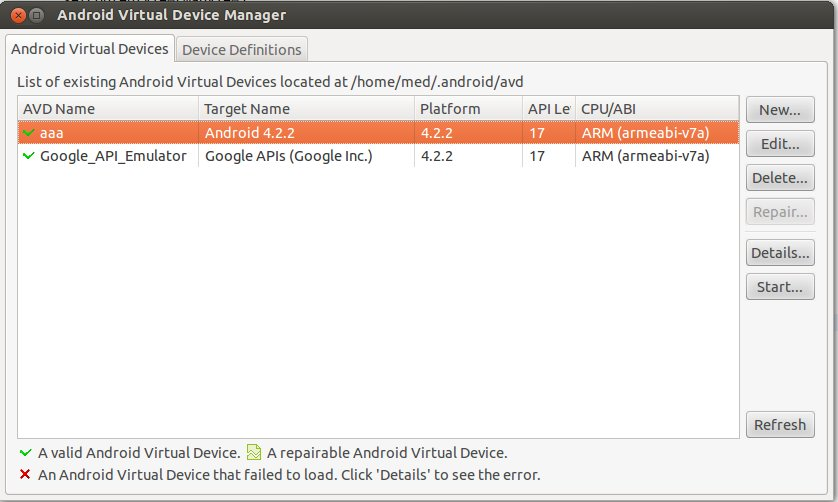
\includegraphics[scale=0.4]{pics/emulator_nastaveni.jpg}
\caption{Správně nastavený emulátoru je na druhém řádku}
\end{center}
\end{figure}
\paragraph{}
Balíček obsahuje vše nezbytné včetně emulátoru. Ke správě, spuštění a nastavení SDK slouží položka v menu \textbf{Window} $\rightarrow$ \textbf{Android SDK Manager}, ke správě emulátoru potom \textbf{Window} $\rightarrow$ \textbf{Android Virtual Device Manager}. K bezproblémovému chodu aplikace v emulátoru je potřeba nastavit jako cílové prostředí \texttt{Google APIs} v poslední verzi (17).
\paragraph{}
Nejnovější verze \texttt{Google API} v nabídce pravděpodobně nebude. K její instalaci je třeba otevřít \textbf{Window} $\rightarrow$ \textbf{Android SDK Manager} a doinstalovat ho. 
\begin{figure}[hb]
\begin{center}
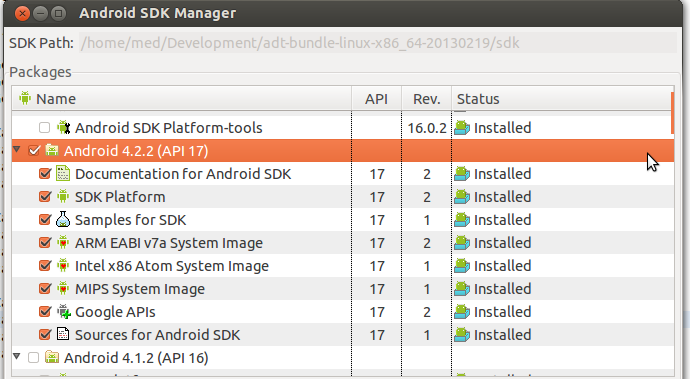
\includegraphics[scale=0.5]{pics/SDK_manager.png}
\caption{Označené balíčky je potřeba doinstalovat}
\end{center}
\end{figure}
\paragraph{}
Pro spuštění aplikace \texttt{Mapa Kamer} v emulátoru je potřeba ještě nastavit souřadnice GPS. To se musí udělat ručně, protože emulátor nemá žádné fyzické GPS zařízení. ze to udělat dvěma způsoby:
\begin{itemize}
\item Ruční nastavení v DDMS:
\begin{itemize}
\item \textbf{Window} $\rightarrow$ \textbf{Open Perspective} $\rightarrow$ \textbf{DDMS},
\item označit emulátor a v záložce \textbf{Emulator Control} nastavit souřadnice,
\item potvrdit tlačítkem \textbf{Send}.
\end{itemize}
\begin{figure}[hb]
\begin{center}
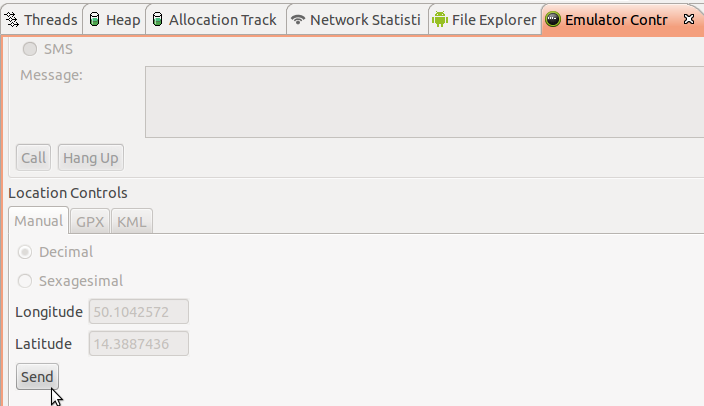
\includegraphics[scale=0.3]{pics/ddms.png}
\caption{Označené balíčky je potřeba doinstalovat}
\end{center}
\end{figure}
\item Pomocí telnetu:
\begin{itemize}
\item otevřít konzoli,
\item připojit zařízení: \texttt{telnet localhost 5554},
\item nastavit souřadnice: \texttt{geo fix 13.24 52.31}.
\end{itemize}
\end{itemize}
Je celkem jedno který z těchto způsobů je použit. Po správném nastavení souřadnic by se měl emulátor chovat jako mobilní zařízení v poloze nastavené těmito souřadnicemi. \textbf{Pozor}: nastavením GPS souřadnic není v zařízení "zapnut" GPS modul. GPS se zapíná v nastavení (\textbf{Menu} $\rightarrow$ \textbf{Settings} $\rightarrow$ \textbf{Location access} $\rightarrow$ \textbf{GPS satellites}). 

\section{Projekt Osmdroid}
V \texttt{Android SDK} existuje mapová podpora pro \texttt{Google Maps}, protože \texttt{Android} patří také společnosti \texttt{Google}. Pro použití \texttt{OpenStreetMap} v aplikaci existuje více možností, kromě námi použitého \texttt{Osmdroid} lze použít například renderovací knihovnu \texttt{MapsForge}\footnote{http://code.google.com/p/mapsforge/}.
\paragraph{}
Balíček \texttt{Osmdroid} umožňuje používání nativních metod pro zobrazování \texttt{Google Maps} k zobrazování dat z projektu \texttt{OpenStreetMap}. V některých případech, jako je třeba zobrazení mapy, její vycentrování nebo nastavení hladiny zoom, se používají metody knihovny \texttt{Osmdroid} přesně jako ekvivalentní metody z balíčku \texttt{google.maps}. V některých jiných případech jsou třídy poněkud odlišné. Příkladem může být třeba zobrazení markerů (třída \texttt{ItemizedOverlay}). V některých případech nám možnosti hotových tříd nestačily a požadovanou funkčnost jsme museli dopsat sami. Stalo se nám to například u zobrazení obrázku v informačním okně vyskakujícím při poklepání na marker v mapě. Pro tento účel jsme vytvořili třídu \texttt{ImageOverlayItem}.
\paragraph{}
Od používání \texttt{OpenStreetMap} na úkor \texttt{Google Maps} jsme si slibovali možnost využití vrstvy \texttt{surveillance} z databáze \texttt{OpenStreetMap}, která obsahuje poměrně velké množství kamer sledujících veřejný prostor a která byla použita ve webové aplikaci Mapa Kamer a z velké míry i dopl\v{n}ována díky aktivitám sdružení  IuRe. K zobrazování vrstvy jsou ve webové aplikaci použity \texttt{OpenLayers}, které ale neexistují ve verzi pro mobilní zařízení, jedině v prohlížeči. Pokoušeli jsme se nalézt nějaké řešení jak použít data z této vrstvy a nakonec jsme se rozhodli pro export dat z databáze \texttt{OpenStreetMap} do lokální databáze na našem serveru. Odtud je možné data normálně zobrazovat v mobilní aplikaci.

\section{Používání aplikace}
Při spuštění aplikace má uživatel na výběr mezi třemi tlačítky:
\begin{itemize}
\item Přidat kameru,
\item Zobrazit mapu kamer,
\item O projektu.
\end{itemize}

\subsection{Přidat kameru}
Nové kamery jsou přidávány přímo do databáze na serveru. Tato databáze se synchronizuje přímo s databází \texttt{OpenStreetMap}. O databázi i samotném nahrávání nové kamery po technické stránce se zmíníme ještě v dalších kapitolách. V této sekci popíšeme co a jak dělat v aplikaci aby byla nová kamera odeslána.
\begin{figure}[!ht]
\begin{center}
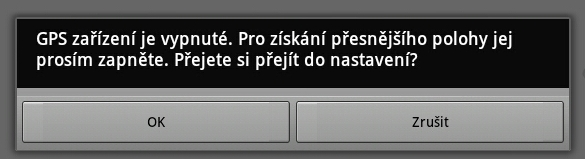
\includegraphics[scale=0.2]{pics/open_GPS.jpg}
\caption{Dialog vybízející k zapnutí GPS}
\end{center}
\end{figure}
\paragraph{}
Při otevření aktivity  aplikace nejprve zkontroluje, zda je zapnutá GPS. Pokud ne, dostane uživatel možnost GPS zapnout a zlepšit tak přesnost zaměření polohy.
\paragraph{} Pokud GPS nezapne, bude poloha určena ze sítě. Poloha je zobrazena na řádku \texttt{GPS lokace}. Do řádku \texttt{popis kamery} uživatel napíše něco o kameře. Mělo by se to týkat faktických věcí, jako například kdo je provozovatelem kamery, upřesnění její polohy nebo například to, jestli kamera pouze zobrazuje, nebo i nahrává záznam. Poslední věc kterou je ke kameře možné přidat je fotografie. Po stisknutí tlačítka je uživatel přesměrován do aplikace fotoaparátu, kterou pořídí snímek. Poté už stačí celý formulář jenom potvrdit a kamera bude přidána do databáze.

\subsection{Zobrazit mapu kamer}
Při spuštění mapy aplikace nejprve zkontroluje, zda je zapnutá GPS. V případě že ano, je na aktuálních souřadnicích vycentrována mapa \texttt{OpenStreetMap}. Pokud GPS zapnutá není, zobrazí se stejný dialog jako v předchozí sekci a uživatel dostane možnost zapnout GPS.
\paragraph{}
Při volbě \textbf{Ano} je uživatel přesměrován do nastavení správy GPS. GPS může, ale nemusí být zapnutá. Pro určení polohy z GPS je použit objekt \texttt{gpsLocListener}. V případě, že se uživatel rozhodne nechat GPS vypnutou (a zvolí \textbf{Ne}), je poloha určována ze sítě pomocí objektu \texttt{networkLocListener}. 
\begin{figure}[!ht]
\begin{center}
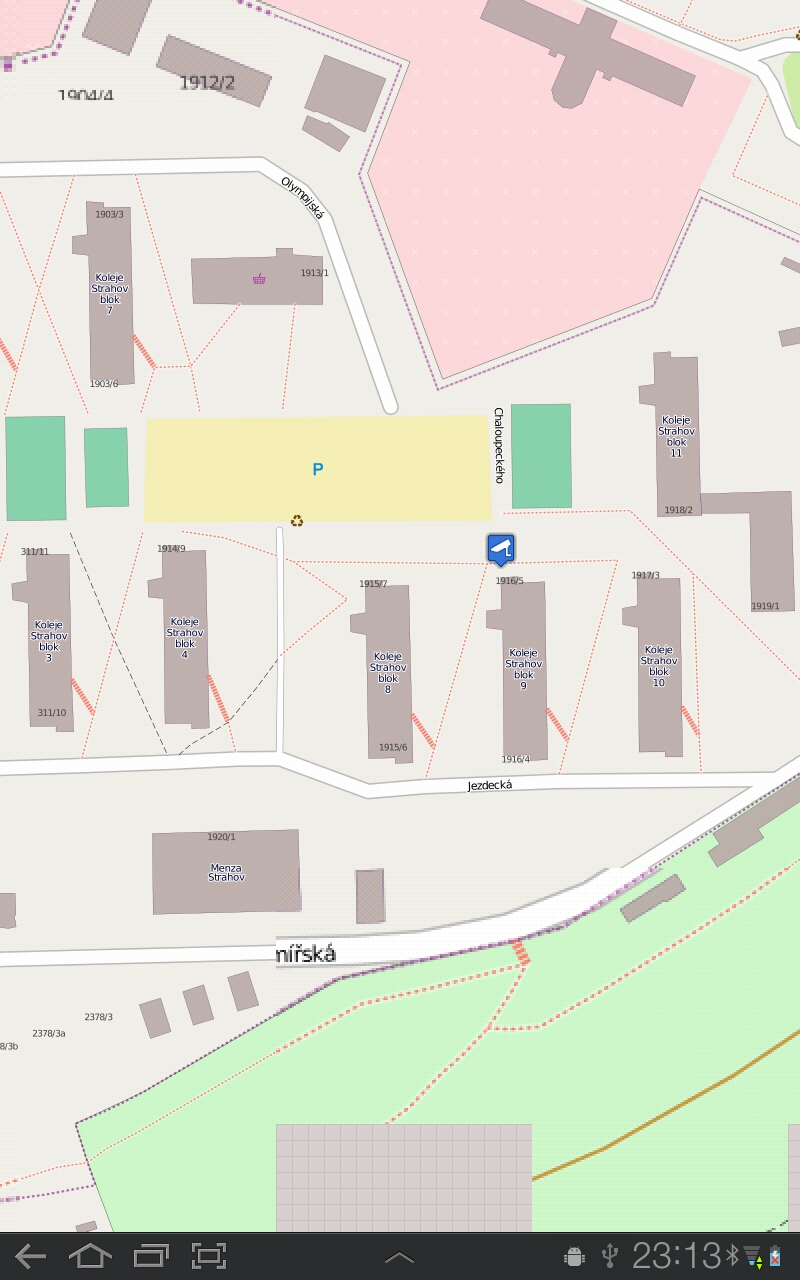
\includegraphics[scale=0.07]{pics/mapa.jpg}
\caption{Mapa vycentrovaná na místě, na kterém jsem psal tuto dokumentaci}
\end{center}
\end{figure}
\paragraph{}
Podklad \texttt{OpenStreetMap} je zobrazen a vycentrován na aktuální pozici. Z databáze jsou poté pomocí příkazu \texttt{SELECT} vytaženy kamery a zobrazeny s markerem se symbolem cctv\footnote{http://mapicons.nicolasmollet.com/markers/offices/cctv/}. Při poklepání na kameru se otevře informační okno s podrobnostmi o kameře. Kromě popisu může obsahovat i fotografii.
\begin{figure}[!ht]
\begin{center}
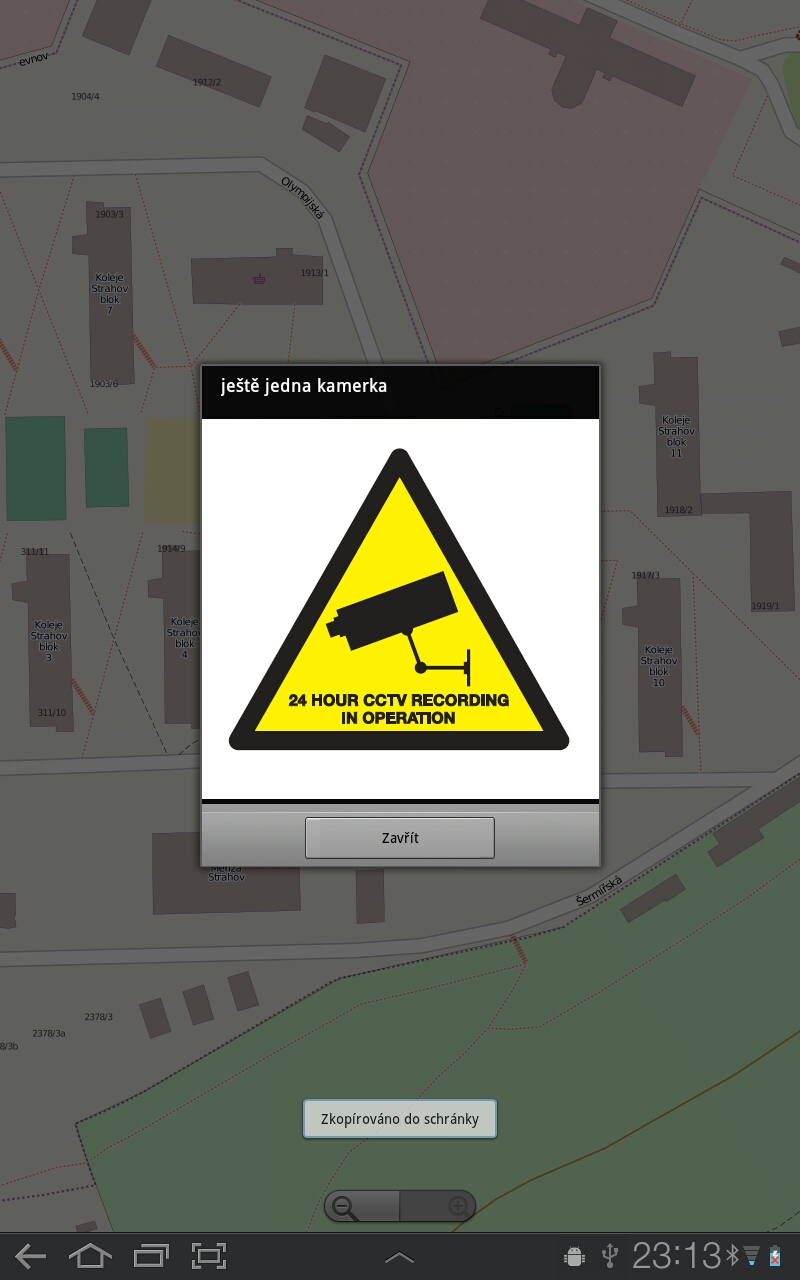
\includegraphics[scale=0.07]{pics/infoWindow.jpg}
\caption{Ukázka informačního okna kamery}
\end{center}
\end{figure}

\subsection{O projektu}
V této záložce se uživatel může dočíst jaké cíle má projekt Mapa kamer, na jakých principech je postaven a také něco o sdružení IuRe a tvůrcích projektu.
\begin{figure}[!ht]
\begin{center}
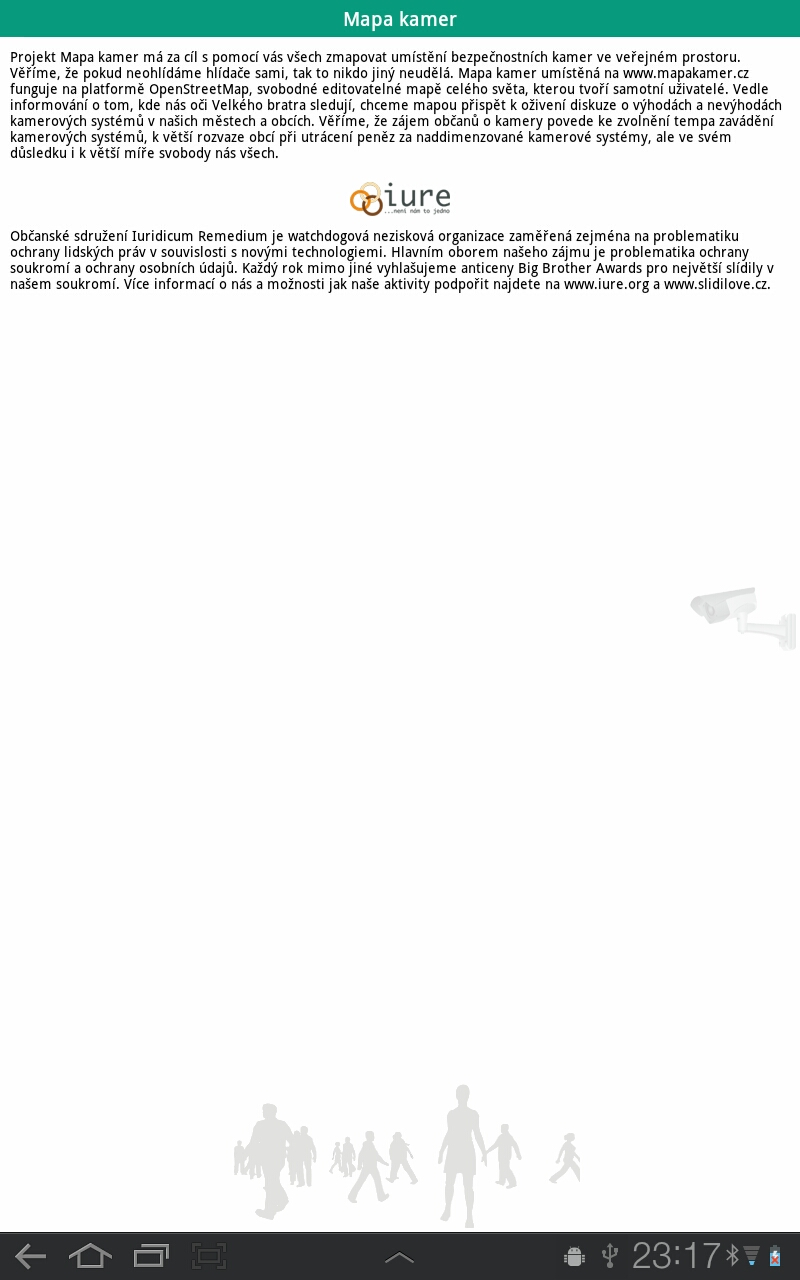
\includegraphics[scale=0.07]{pics/about.jpg}
\caption{Vzhled záložky O projektu (screenshot z tabletu)}
\end{center}
\end{figure}

\section{Základy vývoje aplikací pro Android}
Tvorba aplikace pro systém \texttt{Android} je ve své podstatě hrozně jednoduchá. Každá aplikace má jeden xml soubor pojmenovaný \texttt{Manifest}. Ten obsahuje název balíčku, verze systému pro které je aplikace určená a dále velmi důležitý seznam použitých povolení (\texttt{permissions}) a vlastností (\texttt{features}). Další věci jsou obsaženy v elementu application. Jedná se především o seznam aktivit používaných v aplikaci. Co je to aktivita je vysvětleno dále.
\paragraph{}
Aktivitu si lze představit jako jednu obrazovku mobilního zařízení s tlačítky, nadpisy, menu a vším co k tomu patří. V aplikaci Mapa Kamer je například jednou z aktivit \texttt{HomeActivity}, která obsahuje domácí obrazovku aplikace se třemi tlačítky. Při poklepání na tlačítka se akorát spouští další aktivity, jmenovitě to jsou \texttt{NewCameraActivity}, \texttt{CameraMapActivity} a \texttt{AboutActivity}. 
\begin{figure}[!ht]
\begin{center}
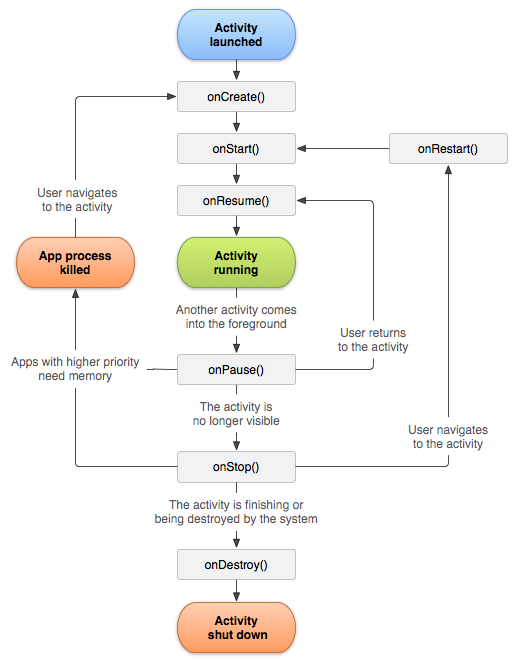
\includegraphics[scale=0.3]{pics/activity_lifecycle.png}
\caption{Životní cyklus aktivity}
\end{center}
\end{figure}
\paragraph{}
Každá aktivita může mít vzhled tvořen buď kódem v jazyce \texttt{Java}, nebo je možné vzhled nastavit pomocí xml souboru v \texttt{res} $\rightarrow$ \texttt{layout}. V prostředí \texttt{Eclipse} je možné xml vytvářet pomocí grafického editoru. 
\paragraph{}
Každá aktivita má svůj životní cyklus. Aktivita může být v jednom ze čtyř základních stavů:
\begin{itemize}
\item \textbf{Aktivní} -- aktivita běží v popředí.
\item \textbf{Pozastavená} -- aktivita je pořád viditelná, ale není aktivní. Chová se stejně jako aktivní aplikace, ale v případě malé paměti zařízení jí systém může zabít.
\item \textbf{Zastavená} -- aktivita je kompletně překryta jinou aktivitou. Když je paměť potřeba jinde, tak jí systém zpravidla zabije.
\item \textbf{Zabitá} -- pokud je pozastavená nebo zastavená aktivita zabita systémem a uživatel ji chce zobrazit, musí být znovu načtena úplně od začátku a uvedena zpět do předchozího stavu.
\end{itemize}
\paragraph{}
Každá aktivita má několik metod, kterými je možné ji uvést do některého z uvedených stavů. Metoda uvádějící aktivitu do určitého stavu má párovou metodu, která tento stav ukončí.
\begin{itemize}
\item \texttt{onCreate} a \texttt{onDestroy}
\item \texttt{onStart} a \texttt{onStop}
\item \texttt{onResume} a \texttt{onPaused}
\end{itemize}